\documentclass[12pt,english]{paper}
\usepackage{mathptmx}
\renewcommand{\ttdefault}{lmtt}
\usepackage[T1]{fontenc}
\usepackage[latin9]{inputenc}
\usepackage{geometry}
\geometry{verbose,tmargin=2cm,bmargin=2cm,lmargin=2cm,rmargin=2cm}
\setlength{\parskip}{\smallskipamount}
\setlength{\parindent}{0pt}
\usepackage{color}
\usepackage{float}
\usepackage{url}
\usepackage{graphicx}
\PassOptionsToPackage{version=3}{mhchem}
\usepackage{mhchem}

\makeatletter

\providecommand{\tabularnewline}{\\}

\usepackage{xcolor}
\usepackage{url}

\makeatother

\usepackage{babel}
\usepackage{listings}
\lstset{backgroundcolor={\color{gray!20}},
basicstyle={\ttfamily\footnotesize}}
\renewcommand{\lstlistingname}{Listing}

\begin{document}

\title{Quantum Espresso Basic Tutorial}


\author{Fadjar Fathurrahman}

\maketitle

\section{Introduction}

Quantum Espresso (QE) package is a collection of various programs
that can be used for first-principles electronic structure calculations
and and materials modeling based on density functional theory, plane
wave basis set, and pseudopotentials \cite{Giannozzi2009}.

In this tutorial we will use QE version 5.2.1. The directory name
is \texttt{espresso-5.2.1}. The packages has been compiled for you.
The binaries or executables can be found in \texttt{espresso-5.2.1/bin}
subdirectory.

There are two main core programs in QE.
\begin{itemize}
\item PWSCF (Plane Wave Self Consistent Field) which is used to carry out
electronic structure calculations based on self-consistent solution
of Kohn-Sham equations. The executable file is named \texttt{pw.x}.
\item CP (Car Parrinello) which is used to carry out Car-Parrinello molecular
dynamics simulation. The executable file is named \texttt{cp.x}.
\end{itemize}
Besides these programs, QE also contains other programs which can
be used to do more specialized calculations.
\begin{itemize}
\item \texttt{PostProc}: to handle various post-processing
\item \texttt{PHonon}: for calculating vibrational properties
\item \texttt{PWneb}: for calculating reaction path and activation energy
\item \texttt{PWcond}: for calculating ballistic conductance
\item \texttt{XSPECTRA}: for calculation of X-ray absorption spectra
\end{itemize}
In this tutorial, we will describe basic usage of PWSCF and several
post processing programs.

PWSCF need several things to do the calculation.
\begin{itemize}
\item Input file. This file is in plain text format and it can be named
as you want. In this input file we specified the molecular or crystalline
structure of the system that we want to calculate and various parameters
for the calculation.
\item Pseudopotential files for each atomic species. These files usually
have extension \texttt{UPF}. They can be found in various sources
in the web or you can generate them by yourself.
\end{itemize}
General format of PWSCF input that will be used in this tutorial is
as follows.

\begin{lstlisting}
&CONTROL
...
/

&SYSTEM
...
/

&ELECTRONS
...
/

&IONS
...
/

ATOMIC_SPECIES
Atom1  Mass1  Pseudo1
Atom2  Mass2  Pseudo2
....

ATOMIC_POSITIONS  units
Atom1  x1  y1  z1
Atom2  x2  y2  z2
....

K_POINTS options
...
\end{lstlisting}



\section{Example: molecular systems}


\subsection{$\ce{N2}$ molecule: SCF calculation}


\subsubsection{Input file}

First, we will do a total energy calculation of $\ce{N2}$ molecule.
To get total energy, we must solve Kohn-Sham equations via a self
consistent field (SCF) algorithm. The example input file for this
calculation is given in \texttt{PWINPUT\_scf}. We will examine the
content of the input file first.

\begin{lstlisting}
&CONTROL
  calculation = 'scf'
  restart_mode = 'from_scratch'
  pseudo_dir = './pseudo'
  outdir = './tmp'
/
\end{lstlisting}

\begin{itemize}
\item \texttt{calculation = 'scf'} means that we want to do a total energy
calculation via self consistent field algorithm. This calculation
can be referred to as single point calculation because we only do
the calculation for one atomic configuration.
\item \texttt{restart\_mode = 'from\_scratch'} means that we want to do
the calculation from the beginning. If you want to restart from a
previous calculation you can specify \texttt{restart\_mode = 'restart'}.
\texttt{'from\_scratch'} is the default value, so if you don't want
to restart a calculation you can simply remove this line from the
input file.
\item \texttt{pseudo\_dir = './pseudo'} is used to specify the path for
pseudopotential files. In our case we place the pseudopotential file
in the directory named \texttt{pseudo} under the current working directory.
You need to change this if you place the pseudopotential files in
other directory.
\item \texttt{outdir = './tmp'} is used to specify directory for temporary
files used by PWSCF. In this case, we specifiy a directory named \texttt{tmp}
under the current directory as the \texttt{outdir}. If this directory
is not present, PWSCF will create it in the runtime.
\end{itemize}
\begin{lstlisting}
&SYSTEM
  ibrav = 1
  a = 15.0
  ntyp = 1
  nat = 2
  ecutwfc = 30.0
  nbnd = 8
/
\end{lstlisting}

\begin{itemize}
\item \texttt{ibrav = 1} means that we used simple cubic lattice for our
calculation. For other lattice we need to specify other values. The
details can be found in PWSCF input documentation \cite{pwscf-doc}.
\item \texttt{a = 15.0} is used to specify lattice parameter for simple
cubic lattice that we used. Here, we used the value 15 angstrom for
the lattice parameter.
\item \texttt{ntyp = 1} means that there is only 1 atom type (i.e. only
nitrogen) in our system ($\ce{N2}$ molecule).
\item \texttt{nat = 2} means that there are two atoms in our system.
\item \texttt{ecutwfc = 30.0} means that we used 30 Ry cutoff energy for
wave function expansion. Typical \texttt{ecutwfc} value ranges between
20-100 Ry. The bigger the value of \texttt{ecutwfc} the more accurate
our calculation. However, it will also take more computational resource.
Here we take a rather small \texttt{ecutwfc} value to get a quick
result.
\item \texttt{nbnd = 8} means that we include 8 bands or orbitals in our
calculation. For $\ce{N2}$ molecule, we have 5 valence electrons
for each N atom. So, there are $2\times5=10$ electrons in our system.
Each band or orbital will be occupied by 2 electrons, so we need at
least 5 bands for our calculation. Here, we also include 3 unoccupied
bands in our calculation. If you don't need to know information about
unoccupied bands, you can simply specify \texttt{nbnd = 5} or leave
it to the default value (which is 5 in this case). In the output file,
the value \texttt{nbnd} is also referred to as number of Kohn-Sham
states.
\end{itemize}
\begin{lstlisting}
&ELECTRONS
  electron_maxstep = 150
  mixing_beta = 0.5
/
\end{lstlisting}

\begin{itemize}
\item \texttt{electron\_maxstep = 150} means that we set the maximum SCF
iteration to 150. The default value is 60. For a rather difficult
system we might need more SCF iteration. You may set this number to
larger value such as 200 or so. However, it is not recommended to
set this value to more than 200. If the SCF does not converge after
many iterations it means that there is a problem with your system.
In this case it is better to reduce the value of \texttt{mixing\_beta}
or use different algorithm for charge mixing or diagonalization.
\item \texttt{mixing\_beta = 0.5} means that we specify the value of 0.5
for charge mixing parameter. Its value ranges from 0.0 to 1.0. The
default value is 0.7. For simple systems, larger value will give faster
SCF convergence. For more difficult systems we might need to reduce
the value of \texttt{mixing\_beta}.
\end{itemize}
\begin{lstlisting}
ATOMIC_SPECIES
N   14.00  N.pbe-kjpaw.UPF
\end{lstlisting}

\begin{itemize}
\item In this part we specify information about atomic species or types
present in our system. We need to specify atomic symbol, atomic mass,
and pseudopotential file associated with each species. In our present
case, we need to specify only one atom type, i.e. nitrogen.
\end{itemize}
\begin{lstlisting}
ATOMIC_POSITIONS angstrom
N      7.50000000       7.50000000       7.50000000
N      7.50000000       7.50000000       8.50000000
\end{lstlisting}

\begin{itemize}
\item In this part we specify atomic coordinates of our system. The coordinates
can be given either in angstrom, bohr, or crystal (fractional). In
the present case, we specify two N atoms and the coordinates are given
in angstrom. One atom is located at the center of the box. Another
atom is located at 1.0 angstrom away from the first atom. We have
chosen the geometry such that the N--N bond is located along the $z$-axis.
\end{itemize}
\begin{lstlisting}
K_POINTS gamma
\end{lstlisting}

\begin{itemize}
\item In this part we specify the scheme for $k$-points sampling. For modeling
molecular system we should choose to sample only $\Gamma$ point.
This is done by specifying \texttt{gamma} option after \texttt{K\_POINTS}.
\end{itemize}

\subsubsection{Visualizing the input file}

Before executing the PWSCF, it is customary to visualize the input
file first. This is useful to make sure that we have specified the
desired atomic coordinates. It also can detect other errors related
to the molecular structure. In this tutorial, we will use Xcrysden
program \cite{Kokalj2003} to visualize the input file of PWSCF. From
terminal you can use the following command

\begin{lstlisting}
xcrysden --pwi PWINPUT_scf
\end{lstlisting}


A dialog box as shown in Figure \ref{fig:dia1} may appear.

\begin{figure}[H]
\noindent \begin{centering}
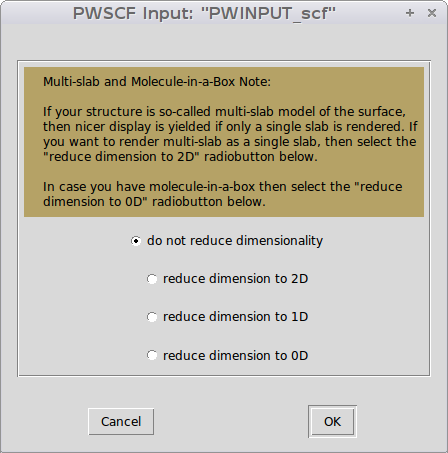
\includegraphics[scale=0.5]{images/RedDimens}
\par\end{centering}

\caption{A dialog box that appears when visualizing PWSCF input. \label{fig:dia1}}


\end{figure}

\begin{itemize}
\item \texttt{do not reduce dimensionality} is the default choice. You must
choose this to visualize 3D periodic systems such as crystalline solid.
\item \texttt{reduce dimension to 2D} is the suitable choice for systems
which have periodicity in two dimensions such as graphene and slab
(surface).
\item \texttt{reduce dimension to 1D} is the suitable choice for systems
which have periodicity in one dimension such as polymer, nanotube,
and nanowire.
\item \texttt{reduce dimension to 0D} is the suitable choice for aperiodic
systems or isolated systems such as molecule.
\end{itemize}
For our current system we may choose \texttt{do not reduce dimensionality}
or \texttt{reduce dimension to 0D}. If you choose \texttt{do not reduce
dimensionality}, the molecule will be displayed along with the box.
The appearance of our system may look like Figure \ref{fig:dia2}.

\begin{figure}[H]
\noindent \begin{centering}
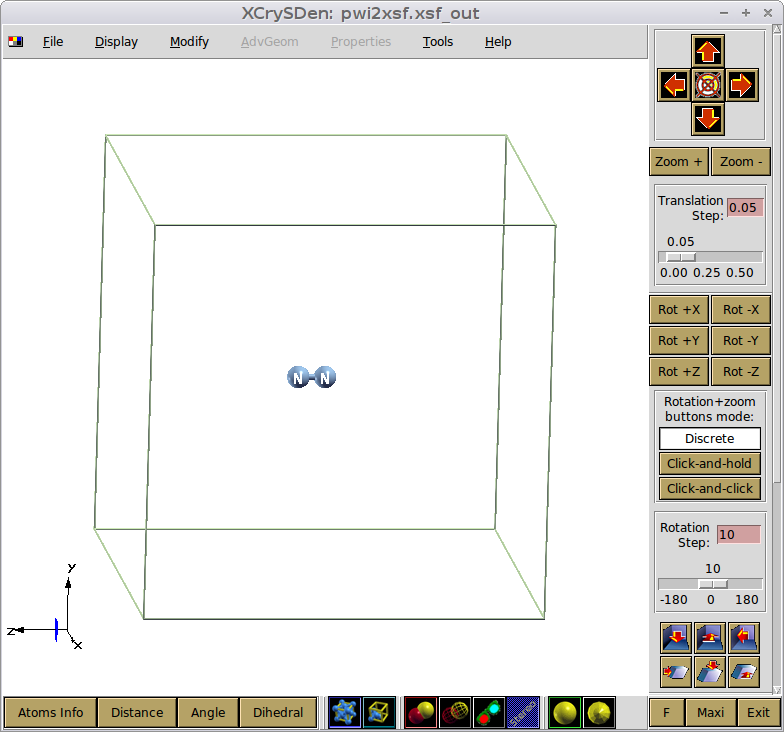
\includegraphics[scale=0.3]{images/N2}
\par\end{centering}

\caption{Appearance of Xcrysden window when displaying \texttt{PWSCF\_input}
of $\ce{N2}$ with \texttt{do not reduce dimensionality}. \label{fig:dia2}}
\end{figure}



\subsubsection{Execution of the program}

The program can be executed by invoking the following command in the
terminal

\begin{lstlisting}
$PATH_TO_QE/pw.x < PWINPUT_scf > LOG_scf &
\end{lstlisting}


If you compiled QE with MPI, you can run PWSCF using more than one
processor. For example, if you want to use 8 processors, you can use
the following command

\begin{lstlisting}
mpirun -np 8 $PATH_TO_QE/pw.x < PWINPUT_scf > LOG_scf &
\end{lstlisting}


You need to change \texttt{\$PATH\_TO\_QE} to your local QE installation
directory. If you have added this directory to the environment variable
\texttt{\$PATH}, you can simply type \texttt{pw.x < PWINPUT\_scf >
LOG\_scf}.

In the above command we have specified the output to be written in
the file \texttt{LOG\_scf}. You can choose other name for the output
file.


\subsubsection{Output file}

After sucessful execution, you may now look into the output file \texttt{LOG\_scf}.
Most part of the output file is self-explanatory. One important part
of the output that you often need is the following part.

\begin{lstlisting}
     bravais-lattice index     =            1
     lattice parameter (alat)  =      28.3459  a.u.
     unit-cell volume          =   22775.6292 (a.u.)^3
     number of atoms/cell      =            2
     number of atomic types    =            1
     number of electrons       =        10.00
     number of Kohn-Sham states=            8
     kinetic-energy cutoff     =      30.0000  Ry
     charge density cutoff     =     120.0000  Ry
     convergence threshold     =      1.0E-06
     mixing beta               =       0.5000
     number of iterations used =            8  plain     mixing
     Exchange-correlation      =  SLA  PW   PBX  PBC ( 1  4  3  4 0 0)
\end{lstlisting}


This part contains some input parameters that we have speficied in
the input file such as Bravais lattice type (\texttt{ibrav}) and lattice
parameter (\texttt{a}). Values for other variables that are not set
in the input file are deduced by PWSCF.

The following part of the output file \texttt{LOG\_scf} shows the
progress of SCF iteration.

\begin{lstlisting}
     Self-consistent Calculation

     iteration #  1     ecut=    30.00 Ry     beta=0.50
     Davidson diagonalization with overlap
     ethr =  1.00E-02,  avg # of iterations =  7.0

     negative rho (up, down):  5.067E-03 0.000E+00

     total cpu time spent up to now is        5.6 secs

     total energy              =     -56.31174606 Ry
     Harris-Foulkes estimate   =     -56.45866183 Ry
     estimated scf accuracy    <       0.27629890 Ry

     iteration #  2     ecut=    30.00 Ry     beta=0.50
....
\end{lstlisting}


The following part shows the end of self consistent iteration.

\begin{lstlisting}
     End of self-consistent calculation

          k = 0.0000 0.0000 0.0000 ( 31539 PWs)   bands (ev):

   -29.8582 -12.7606 -12.4912 -12.4911 -10.2086  -0.6822  -0.6820  -0.5092

     highest occupied, lowest unoccupied level (ev):   -10.2086   -0.6822
\end{lstlisting}


This part also shows the information about band (orbital) energies
of our system in eV. In our case, it will shows 8 band energies. It
also indicates the HOMO and LUMO levels.

The following part shows the information about total energy of our
system. For most purposes, this is the most important output.

\begin{lstlisting}
!    total energy              =     -56.34181959 Ry
     Harris-Foulkes estimate   =     -56.34181965 Ry
     estimated scf accuracy    <       0.00000033 Ry

     total all-electron energy =      -218.939422 Ry

     The total energy is the sum of the following terms:

     one-electron contribution =     -93.16252129 Ry
     hartree contribution      =      47.83652622 Ry
     xc contribution           =     -10.81473725 Ry
     ewald contribution        =      16.46583375 Ry
     one-center paw contrib.   =     -16.66692103 Ry
\end{lstlisting}


Note that you also can extract a line containing total energy information
from the output file \texttt{LOG\_scf} by using the following command:
\begin{lstlisting}
grep ! LOG_scf
\end{lstlisting}


This command will search and display lines that contains the character
!. In this case it will display the line that also contains total
energy information.

\begin{lstlisting}
!    total energy              =     -56.34181959 Ry
\end{lstlisting}



\subsubsection{Convergence study}

It is good practice to do convergence study before doing into more
serious calculations. In a convergence study we do a series of calculations
by varying some input variables and observe how the output changes.
One of important input variable is \texttt{ecutwfc}. You may want
to vary the value of \texttt{ecutwfc} and observe how the total energy
changes as function of \texttt{ecutwfc}.


\subsection{$\ce{N2}$ molecule: geometry optimization}

In this subsection, we will do a geometry optimization or relaxation
of $\ce{N2}$ molecule. The input file for this calculation is \texttt{PWINPUT\_relax}.
The content is similar to the \texttt{PWINPUT\_scf}. The most important
changes are described as follows.

\begin{lstlisting}
&CONTROL
  calculation = 'relax'
  restart_mode = 'from_scratch'
  pseudo_dir = './pseudo'
  outdir = './tmp'
/
\end{lstlisting}

\begin{itemize}
\item For a geometry optimization calculation, we need to specify \texttt{calculation
= 'relax'} instead of \texttt{'scf'}. For a more difficult geometry
optimization which takes more than 50 steps you may want to add new
variable \texttt{nstep} and set it to a rather large number such as
\texttt{nstep = 1000} in the \texttt{\&CONTROL} namelist.
\end{itemize}
\begin{lstlisting}
&IONS
  ion_dynamics = 'bfgs'
/
\end{lstlisting}

\begin{itemize}
\item In this part we specify the algorithm to be used for geometry optimization.
In this case, we choose the BFGS (Broyden-Fletcher-Goldfarb-Shanno)
algorithm.
\end{itemize}
You can run PWSCF as usual. In our case we will choose \texttt{LOG\_relax}
as the output file.

\begin{lstlisting}
$PATH_TO_QE/pw.x < PWINPUT_relax > LOG_relax &
\end{lstlisting}


One important part of the output file is the following.

\begin{lstlisting}
     BFGS Geometry Optimization

     number of scf cycles    =   1
     number of bfgs steps    =   0

     energy   new            =     -56.3418195913 Ry

     new trust radius        =       0.5000000000 bohr
     new conv_thr            =       0.0000010000 Ry


ATOMIC_POSITIONS (angstrom)
N        7.500000000   7.500000000   7.235411396
N        7.500000000   7.500000000   8.764588604
\end{lstlisting}


A geometry optimization contains several SCF calculations. You can
get the converged total energies of the structure during geometry
optimization by using the following command.

\begin{lstlisting}
grep ! LOG_relax
\end{lstlisting}
and you will get the following output on the terminal

\begin{lstlisting}
!    total energy              =     -56.34181959 Ry
!    total energy              =     -56.04773937 Ry
!    total energy              =     -56.38958712 Ry
!    total energy              =     -56.41785625 Ry
!    total energy              =     -56.42197771 Ry
!    total energy              =     -56.42284642 Ry
!    total energy              =     -56.42285738 Ry
\end{lstlisting}


You can visualize the result of the geometry optimization using Xcrysden.

\begin{lstlisting}
xcrysden --pwo LOG_relax
\end{lstlisting}


You can choose the same options as you do when visualizing the input
file \texttt{PWINPUT\_scf}. One different small window that may appear
is shown in Figure \ref{fig:DispCoordAsAnim}. If you choose \texttt{Display
All Coordinates as Animation}, the animation showing the change of
molecular geometry during the relaxation is shown.

\noindent \begin{center}
\begin{figure}[H]
\noindent \begin{centering}
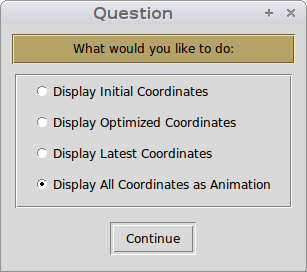
\includegraphics[scale=0.5]{images/DispCoordAsAnim}
\par\end{centering}

\caption{A dialog box that appear when visualizing an optimization output file
of PWSCF.\label{fig:DispCoordAsAnim}}
\end{figure}

\par\end{center}


\subsection{$\ce{N2}$ molecule: visualization of molecular orbitals}

Now, we will describe an example use of post-processing programs in
QE. We will specifically focus on the program \texttt{pp.x}. Using
this program, we can extract some data after main PWSCF calculations
are done. These data include partial and total charge density, potential,
STM images, and wavefunctions or orbitals. In the following example
we will extract the molecular orbitals of $\ce{N2}$.~To be more
precise, we are not actually extracting the molecular orbitals, but
the squared values of these orbitals with their sign. The content
of the input file \texttt{PPINPUT} is as follows.

\begin{lstlisting}
&INPUTPP
  outdir = './tmp'
  plot_num = 7
  lsign = .true.
  filplot = PSI2.dat
  kpoint = 1
  kband = 5
/

&PLOT
  iflag = 3
  output_format = 5
  fileout = 'MO5.xsf'
/
\end{lstlisting}

\begin{itemize}
\item \texttt{outdir = './tmp'} specify the path of temporary directory
of PWSCF calculation. It should be the same as the one specify before
for PWSCF calculation.
\item \texttt{plotnum = 7} means that we want to plot the contribution of
a selected wavefunction to the charge density. Other possible values
of \texttt{plotnum} and their meaning can be found in \texttt{pp.x}
documentation \cite{pp-doc}.
\item \texttt{lsign = .true.} means that we include the sign of the wavefunction.
This option only works for $\Gamma$-point-only calculation. This
is the case for our present calculation.
\item \texttt{filplot = PSI2.dat} specify the temporary file that contains
the data that we extract. In this case we name it \texttt{PSI2.dat}.
This file can used for further analysis. If you don't do more analysis
you can delete this file.
\item \texttt{kpoint = 1} specify the index of $k$-point of the wavefunction
that we want to plot. In the present case we only have one $k$-point
($\Gamma$-point), so we specify \texttt{kpoint = 1}.
\item \texttt{kband = 5} specify index of the band or orbital that we want
to plot. Remember that we specify nbnd = 8 in our previous PWSCF calculations,
so kband can take value from 1 to 8. Also remember that $\ce{N2}$
have 10 valence electrons, so specifying \texttt{kband = 5} means
that we want to plot the highest occupied molecular orbital (HOMO).
\item \texttt{iflag = 3} means that we want to extract 3D data.
\item \texttt{output\_format = 5} means that we want the output to be in
Xcrysden's XSF format. Note that, other formats are also supported.
For more details, please consult the \texttt{pp.x} documentation \cite{pp-doc}.
\item \texttt{fileout = 'MO5.xsf'} specify the name of the output file.
\end{itemize}
The command to execute \texttt{pp.x} is similar to the command to
execute \texttt{pw.x}.

\begin{lstlisting}
$PATH_TO_QE/pp.x < PPINPUT
\end{lstlisting}


Note that, we don't redirect the standard output of \texttt{pp.x}
to a file. If you want to redirect it to a file you can append \texttt{>
LOG\_pp} at the end of the above command.

After successful execution you should find the \texttt{MO5.xsf} file
in the working directory. You can open it using Xcrysde

\begin{lstlisting}
xcrysden --xsf MO5.xsf
\end{lstlisting}


After Xcrysden display the $\ce{N2}$ molecule you can visualize MO
by choosing the menu \texttt{Tools} $\rightarrow$ \texttt{Data Grid}.
A small dialog box as show in Figure \ref{fig:dia3} will then appear.
You can just click OK.

\begin{figure}[H]
\noindent \begin{centering}
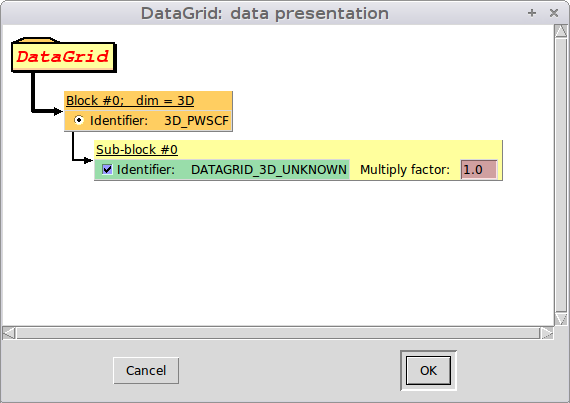
\includegraphics[scale=0.3]{images/DatagridWindow}
\par\end{centering}

\caption{Data grid dialog box \label{fig:dia3}}
\end{figure}


After clicking OK, a window like shown in Figure \ref{fig:dia4} will
appear. You can give the \texttt{Isovalue} a relatively small number
and check the \texttt{Render +/- isovalue}. After you have specified
the \texttt{Isovalue} you can click \texttt{Submit} button and see
the visualization of the orbital on the main Xcrysden window. Note
that you can find the maximum and mininum grid values in this window.
You must be careful when checking the \texttt{Render +/- isovalue}.
If the specified isovalue lies beyond the maximum and mininum grid
values, Xcrysden will complain about it.

\begin{figure}[H]
\noindent \begin{centering}
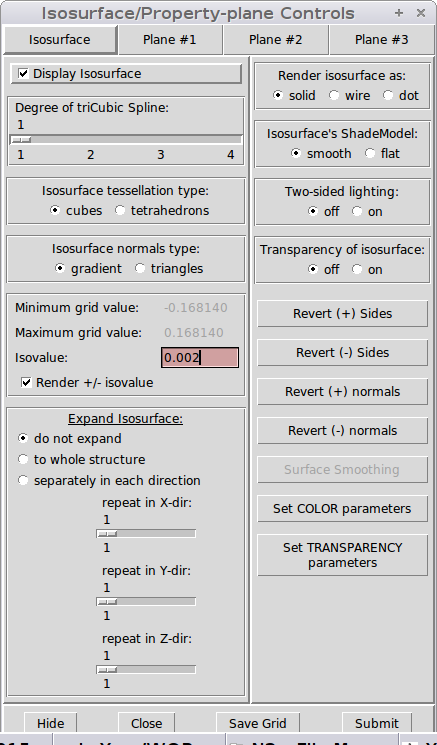
\includegraphics[scale=0.3]{images/IsosurfaceWindow}
\par\end{centering}

\caption{Isosurface control in Xcrysden \label{fig:dia4}}
\end{figure}


Example of the resulting images are shown in Figure \ref{fig:N2-homo-lumo}
for HOMO (\texttt{kband=5}) and LUMO (\texttt{kband=6}).

\begin{figure}[H]
\noindent \begin{centering}
\begin{tabular}{|c|c|}
\hline
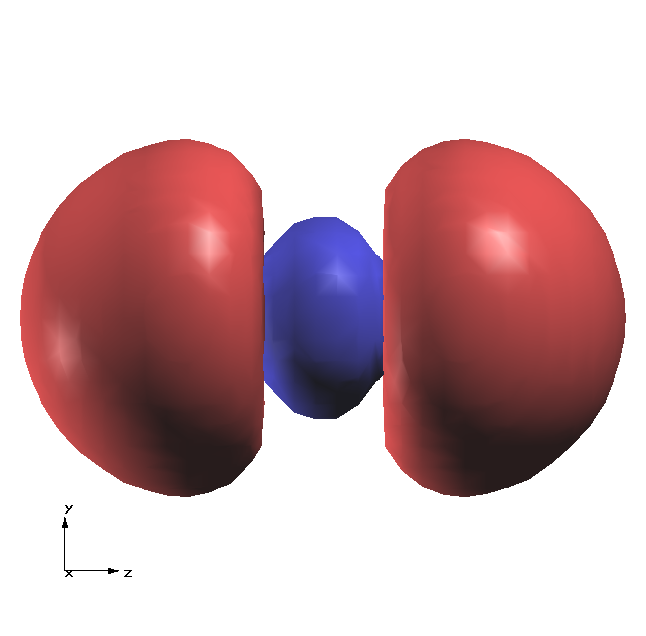
\includegraphics[scale=0.2]{images/N2_MO5} & 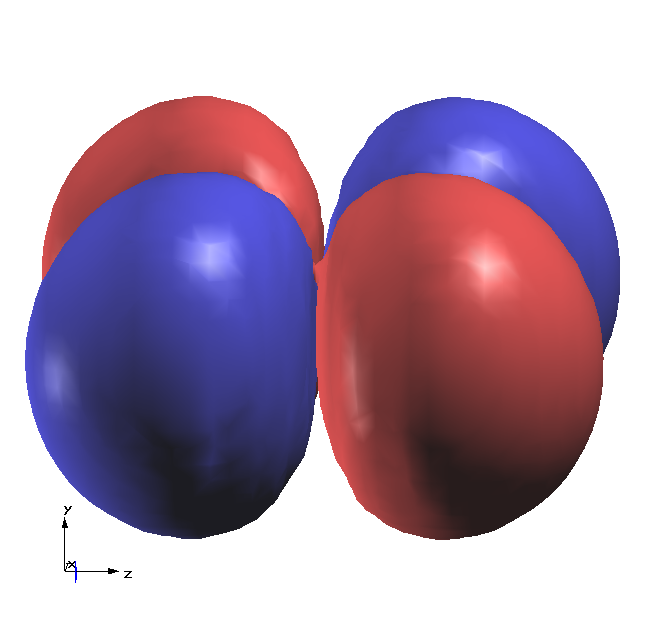
\includegraphics[scale=0.2]{images/N2_MO6}\tabularnewline
\hline
HOMO & LUMO\tabularnewline
\hline
\end{tabular}
\par\end{centering}

\caption{Visualization of HOMO and LUMO of $\ce{N_{2}}$.\label{fig:N2-homo-lumo}}
\end{figure}



\section{Example: bulk systems}


\subsection{Copper: SCF calculation}

The input variables in \texttt{\&CONTROL} namelist are the same as
in the case of $\ce{N2}$. Meanwhile, the content of the \texttt{\&SYSTEM}
namelist is as follows.

\begin{lstlisting}
&SYSTEM
  ibrav = 2
  celldm(1) = 6.73
  nat = 1
  ntyp= 1
  ecutwfc = 30.0
  occupations = 'smearing'
  smearing = 'gaussian'
  degauss = 0.02
/
\end{lstlisting}


Notice the following important difference:
\begin{itemize}
\item We have used FCC lattice by specifying \texttt{ibrav = 2}.
\item \texttt{celldm(1) = 6.73} specify the lattice parameter in atomic
unit (bohr). Notice that you also can specify it by using a = ...
(in angstrom). Conversion factor from bohr to angstrom: 1 bohr = 0.529177...
angstrom
\item The input variable \texttt{occupations = 'smearing'} specifies the
fractional occupation scheme. This scheme is required for metallic
system even though it also can be used for semiconductor and insulator.
If you are unsure about whether your system is metallic or not you
can use this scheme. This scheme can help SCF convergence which is
usually quite difficult in metallic systems. In our present case we
use Gaussian function for smearing by specifying \texttt{smearing
= 'gaussian'}. Other smearing functions that are implemented in PWSCF
are Metfessel-Paxton\texttt{ }(\texttt{'mp'} or \texttt{'m-p'}), Marzari-Vanderbilt
(\texttt{'mv'} or \texttt{'m-v'} or 'cold') and Fermi-Dirac smearing
(\texttt{'fd'} or \texttt{'f-d'}). \texttt{degauss = 0.02} specify
the smearing parameter (electronic temperature) in Ry. It is usually
ranges from 0.00 to 0.10 Ry or so.
\end{itemize}
\begin{lstlisting}
ATOMIC_SPECIES
Cu 63.55 Cu.pbe-kjpaw.UPF

ATOMIC_POSITIONS crystal
Cu 0.0 0.0 0.0

K_POINTS automatic
 8 8 8 0 0 0
\end{lstlisting}

\begin{itemize}
\item Using the specified Bravais lattice, we can define the atomic position
of Cu in the (primitive) unit cell. Here we have defined the coordinates
in \texttt{crystal} coordinate.
\item To sample the $k$-space, we used Monkhorst-Pack scheme by specifying
\texttt{K\_POINTS automatic}. The size of the grid is $8\times8\times8$.
This is specified in the first 3 numbers of the line below. The last
three numbers specify the shift. In the present case we do not shift
the grid and specify the three zeroes as the last three numbers.
\end{itemize}
You can visualize the input file by Xcrysden. The result should be
similar to the one shown in Figure \ref{fig:Cu-crystal}.

\begin{figure}[H]
\noindent \begin{centering}
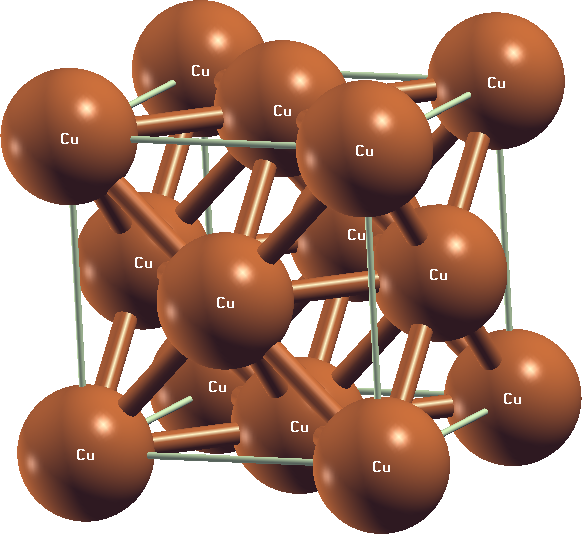
\includegraphics[scale=0.2]{images/Cu_fcc}
\par\end{centering}

\caption{Cu crystal \label{fig:Cu-crystal}}
\end{figure}


You can execute PWSCF as usual and examine the output file.

\begin{lstlisting}
$PATH_TO_QE/pw.x < PWINPUT_scf > LOG_scf
\end{lstlisting}


\textbf{A note about convergence}

As we have mentioned previously, we need to conduct convergence study.
For periodic systems, we usually conduct convergence study with respect
to \texttt{ecutwfc}, k-point sampling and \texttt{degauss} value.


\subsection{Copper: band structure calculation}

After we have done an SCF calculation, we now can do a band structure
calculation. This calculation is done by solving one-particle Schrodinger
equation with constant potential. This potential is the same as the
Kohn-Sham potential that we obtained from a converged SCF calculation.
Band structure calculation is usually done with certain $k$-points
that lies on the path that crosses several high-symmetry points of
the Brillouin zone. In the present case of FCC lattice, we will choose
the following path: $\mathrm{W}\rightarrow\mathrm{L}\rightarrow\Gamma\rightarrow\mathrm{X}\rightarrow\mathrm{W}\rightarrow\mathrm{K}$.
We need to know the coordinate of these high symmetry points. In this
example, we will use Python library ASE (Atomic Simulation Environment)
\cite{Bahn2002} to generate the $k$-point path. An example script
is given in \texttt{gen\_kpts.py}. The full source of the script is
given in Appedix \ref{sec:k-gen-script}.

The script can be executed by issuing the following command on terminal:

\begin{lstlisting}
python gen_kpts.py
\end{lstlisting}


The output of the program can be copied into the PWSCF input file.
Here, we will use \texttt{PWINPUT\_bands} as the name of the PWSCF
input file for band structure calculations. The specification of the
\texttt{K\_POINTS} in \texttt{PWINPUT\_bands} should look like this

\begin{lstlisting}
K_POINTS crystal
60
0.50000000 0.25000000 0.75000000  1.0
0.50000000 0.27083333 0.72916667  1.0
....
\end{lstlisting}
Note that we have specified \texttt{nbnd = 8} in the \texttt{\&SYSTEM}
namelist.

You can execute PWSCF as usual

\begin{lstlisting}
$PATH_TO_QE/pw.x < PWINPUT_bands > LOG_bands
\end{lstlisting}


The standard output file is redirected to \texttt{LOG\_bands}. After
the calculation is finished, you can examine the file \texttt{LOG\_bands}.
The most important part is the following.

\begin{lstlisting}
     End of band structure calculation

          k =-1.0000 0.5000 0.0000 (   208 PWs)   bands (ev):

    12.1282  12.7725  12.7725  14.1620  14.9791  23.0834  23.0834  25.5436

          k =-0.9583 0.5000 0.0417 (   208 PWs)   bands (ev):

    12.1442  12.7434  12.7862  14.1615  14.9590  22.7075  22.8950  25.9793
....
\end{lstlisting}


As you may notice, at the end of the band structure calculation, PWSCF
will give the $k$-point and band energies at that $k$-point. In
our case there will be 60 $k$-points and 8 band energies for each
$k$-points. Using this information we can already construct the band
structure. However, this task is quite tedious as we need to parse
the output file and calculate the length of $k$-vector for each $k$-points.
You can make a script to do these tasks.

Alternatively we can use post-processing program \texttt{bands.x}
to collect the bands and give us a file that is easier to be plotted.
An example input file for \texttt{bands.x} is given in the file \texttt{bands.inp}.
The content of the file is very simple: we only need to specify \texttt{outdir}
which is the same as the one we used for \texttt{pw.x} and leave other
variables to their default values.

\begin{lstlisting}
&BANDS
  outdir = './tmp'
/
\end{lstlisting}


We can execute the \texttt{bands.x} by using the following command:

\begin{lstlisting}
$PATH_TO_QE/bands.x < bands.inp > LOG_collect_bands
\end{lstlisting}


The standard output is given in \texttt{LOG\_collect\_bands}. The
relevant part of this file is the following.

\begin{lstlisting}
     high-symmetry point: -1.0000 0.5000 0.0000   x coordinate   0.0000
     high-symmetry point: -0.5000 0.5000 0.5000   x coordinate   0.7071
     high-symmetry point:  0.0000 0.0000 0.0000   x coordinate   1.5731
     high-symmetry point: -1.0000 0.0000 0.0000   x coordinate   2.5731
     high-symmetry point: -1.0000 0.5000 0.0000   x coordinate   3.0731
     high-symmetry point: -0.7500 0.7500 0.0000   x coordinate   3.4267

     Plottable bands written to file bands.out.gnu
     Bands written to file bands.out
\end{lstlisting}


\texttt{bands.x} detects the 6 high-symmetry points that lies on our
$k$-point path (i.e. $\mathrm{W}\rightarrow\mathrm{L}\rightarrow\Gamma\rightarrow\mathrm{X}\rightarrow\mathrm{W}\rightarrow\mathrm{K}$).
\texttt{bands.x} also gives two other output files, namely \texttt{bands.out}
and \texttt{bands.out.gnu}. The file \texttt{bands.out.gnu} contains
the band structure data that can be plotted using various plotting
programs such as gnuplot, Xmgrace, or even M\$ Excel. Beside these
programs, you can use another post-processing program \texttt{plotband.x}
that is provided by QE.

In this tutorial, we will use Python and matplotlib \cite{Hunter2007}
to produce the band structure plot. This script is given in the file
\texttt{plot\_bands\_gnu.py}. The full listing of the script can be
found in Appendix \ref{sec:plot-band-script}. You can execute the
program by the following command

\begin{lstlisting}
python plot_bands_gnu.py
\end{lstlisting}


You may want to edit the file \texttt{plot\_bands\_gnu.py} to suit
your need and taste. If the execution of the Python script is successful
you can get the band structure as shown in Figure \ref{fig:Cu-bands}.

\begin{figure}[H]
\noindent \begin{centering}
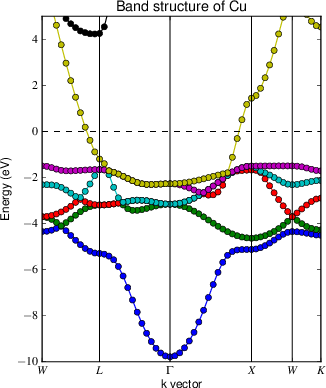
\includegraphics[scale=0.8]{images/Cu_bands_v1}
\par\end{centering}

\caption{Band structure of Cu. \label{fig:Cu-bands}}
\end{figure}



\subsection{Silicon: SCF and band structure calculations}

Silicon cyrstal can be described by FCC lattice with two atom per
unit cell.

\begin{lstlisting}
ATOMIC_POSITIONS  crystal
Si 0.00 0.00 0.00
Si 0.25 0.25 0.25
\end{lstlisting}


We will use lattice parameter of 10.25 angstrom. There will be 8 electrons
in the system, so we need at least 4 bands which can be deduced by
PWSCF by default. Here, we also include 4 extra bands. Also, because
we know that silicon is a semiconductor, we will not use smearing
for this system.

\begin{lstlisting}
&SYSTEM
  ibrav = 2
  celldm(1) = 10.25
  nat = 2
  ntyp= 1
  ecutwfc = 30.0
  nbnd = 8
/
\end{lstlisting}


You can visualize the input that you have prepared. It should look
like the following figure.

\begin{figure}[H]
\noindent \begin{centering}
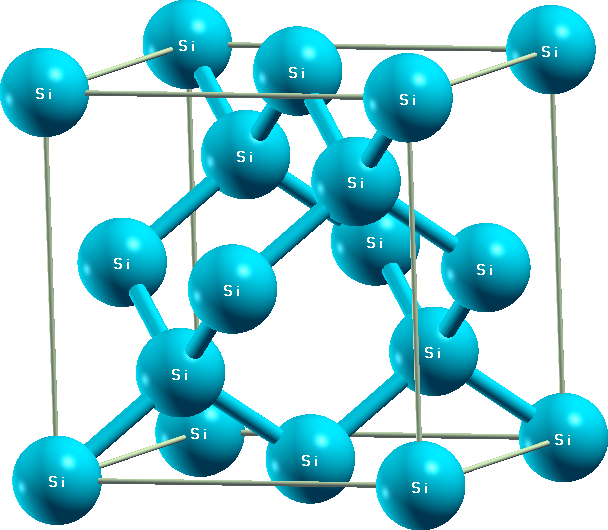
\includegraphics[scale=0.2]{images/Si_fcc}
\par\end{centering}

\caption{Si crystal.}
\end{figure}


The basic work flow is essentially similar to the one we have described
before for copper. If your calculations are successful, you may get
the following band structure. You may use the same $k$-points path
that you have used before when calculating band structure of Cu.

\begin{figure}[H]
\noindent \begin{centering}
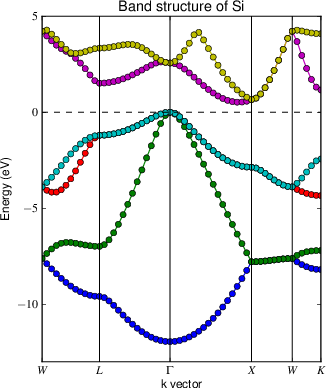
\includegraphics[scale=0.8]{images/Si_bands_v1}
\par\end{centering}

\caption{Band structure of Si.}
\end{figure}



\section{Exercises}

\textbf{Exercise 1 }Try to optimize the geometry of other simple molecules
such as $\ce{NH3}$, $\ce{H2O}$, $\ce{CH4}$, etc. Try also to visualize
the molecular orbitals. You can construct the starting geometries
of these molecules manually or search the coordinates at online database,
such as \url{https://pubchem.ncbi.nlm.nih.gov/search/search.cgi}

\textbf{Exercise 2} Try to calculate the band structure of other crystalline
solids which have FCC structure such as Pd, Pt, Au, Ag, etc. You can
use the same coordinate as the one we have for Cu. For lattice parameters
you can use the lattice parameters for elemental solids that are given
at \url{http://www.webelements.com/} or other sources.

\textbf{Exercise 3} Try to calculate the band structure of other crystalline
solids which have similar structure as Si such as Ge, C (diamond),
GaAs, ZnS, etc. The lattice parameters may be found in standard textbooks
on solid state physics/chemistry.

\rule[0.5ex]{1\columnwidth}{1pt}

\appendix

\section{\label{sec:k-gen-script}Script to generate $k$-points}

The following script is used to generate $k$-points for band structure
calculation.

\begin{lstlisting}[breaklines=true,language=Python,showstringspaces=false,tabsize=2]
from ase.dft.kpoints import *
from ase.units import Bohr
import sys

# Any lattice parameter should work, the important ones are the
# lattice vectors v1, v2, and v3. In this case we used the definition
# of FCC lattice vectors used in PWSCF.
alat = 6.73*Bohr
v1 = [-1,0,1]
v2 = [ 0,1,1]
v3 = [-1,1,0]
cell = 0.5*alat*np.array( [v1, v2, v3] )

# Number of total k-points in the path
NKPT = 60
# Use ase.dft module for obtaining k-points along high symmetry directions
points = ibz_points['fcc']
G = points['Gamma']
X = points['X']
W = points['W']
K = points['K']
L = points['L']
kpts, x, Xkpt = get_bandpath([W, L, G, X, W, K], cell, npoints=NKPT)

# Write kpts in the format understood by PWSCF
# The weights of the k-points are not used, so they can take any value.
# In this case we set them all to 1.0
sys.stdout.write('%d\n' % NKPT)
for ik in range(NKPT):
  sys.stdout.write('%.8f %.8f %.8f  1.0\n' % (kpts[ik,0],kpts[ik,1],kpts[ik,2]))
\end{lstlisting}



\section{\label{sec:plot-band-script}Script to plot band structure}

The following script is used to plot the band structure given the
\texttt{bands.out.gnu} from \texttt{bands.x}.

\begin{lstlisting}[language=Python,tabsize=2]
import numpy as np
import matplotlib.pyplot as plt
from ase.units import Ry

NBANDS   = 8
NKPOINTS = 60

databands = np.loadtxt('bands.out.gnu')

ebands = np.zeros( (NKPOINTS, NBANDS) )
kvec   = np.zeros( (NKPOINTS, NBANDS) )

for ib in range(NBANDS):
  idx1 = (ib)*NKPOINTS
  idx2 = (ib+1)*NKPOINTS
  ebands[:,ib] = databands[idx1:idx2,1]*Ry # convert from Ry to eV
  kvec[:,ib]   = databands[idx1:idx2,0]

# Efermi can be obtained from LOG_scf file. It is calculated when using
# occupation = 'smearing'.
Efermi = 16.4769 # in eV

# If you don't use smearing, Efermi can be taken to be the highest energy
# of the highest occupied band. In this case, uncomment the following two lines
# Nocc = 4  # number of occupied bands
# Efermi = np.max( ebands[:,Nocc-1] )

# Band energy is shifted relative to Efermi
ebands[:,:] = ebands[:,:] - Efermi

# You can set this to match your need
Emin = -10
Emax = 5

# Set the figure size
plt.figure(figsize=(5, 6))
plt.clf()
# Plot the band structure
for ib in range(NBANDS):
  plt.plot( kvec[:,ib], ebands[:,ib], marker='o' )

# You can find the coordinates for Xkpt from standard output of bands.x
# In this tutorial, this file is LOG_collect_bands
Xkpt   = [0.0000, 0.7071, 1.5731, 2.5731, 3.0731, 3.4267]
labelX = ['W', 'L', r'$\Gamma$', 'X', 'W', 'K']

for p in Xkpt:
  plt.plot([p, p], [Emin, Emax], 'k-')
plt.xticks(Xkpt, labelX)

# Plot the horizontal line at y=0
plt.plot([0, Xkpt[-1]], [0, 0], 'k--')

# Set limit for y-axis
plt.ylim( Emin,Emax )
# Set limit for x-axis
plt.xlim( 0, Xkpt[-1] )
# Label for x-axis
plt.xlabel('k vector')
# Label for y-axis
plt.ylabel('Energy (eV)')
# Title of the plot
plt.title('Band structure of Cu')
# Save the resulting figure in pdf format.
# You also can save it in other formats. For example, if you want to use PNG file
# you can simply replace the extension .pdf to .png
plt.savefig('Cu_bands_v1.pdf')
\end{lstlisting}



\section{Tips for generating crystalline structure using \texttt{cif2cell}}

\texttt{cif2cell} is a Python program that can be used to convert
CIF (crystallographic information file) and preparing input file for
various electronic structure programs, including Quantum Espresso.
This program can be found at \url{https://sourceforge.net/projects/cif2cell/}.
You can search CIFs for various crystalline structures at \url{http://www.crystallography.net/search.html}
or other sources. An example use of this program can is as follows.
For example, we want to investigate electronic structure of gallium
nitride (GaN). We can find the CIF of GaN, say with the name \texttt{GaN.cif}.
Also, suppose that we want to build a $3\times3\times3$ supercell
of this tructure. Using cif2cell we can use the following program
to generate the input file for PWSCF.

\begin{lstlisting}
cif2cell -p pwscf --supercell=[3,3,3] --setup-all GaN.cif
\end{lstlisting}


The resulting input file can be found in file GaN.in. The content
of the file will look like this.

\begin{lstlisting}[basicstyle={\scriptsize\ttfamily}]
#************************************************************************************
#*                   Generated by cif2cell 1.2.7 2016-03-17 10:30                   *
#*  T. Bjorkman, Comp. Phys. Commun. 182, 1183-1186 (2011). Please cite generously. *
#*                                                                                  *
#*                                   Ga N   (GaN)                                   *
#*                Wyckoff R W G, Crystal Structures 1, 85-237 (1963)                *
#************************************************************************************

&SYSTEM
  ibrav = 0
  A =    3.18000
  nat = 108
  ntyp = 2
/
CELL_PARAMETERS {alat}
  2.598076211353316  -1.500000000000000   0.000000000000000
  0.000000000000000   3.000000000000000   0.000000000000000
  0.000000000000000   0.000000000000000   4.873584905660377
ATOMIC_SPECIES
  Ga   69.72300  Ga_PSEUDO
   N   14.00650   N_PSEUDO
ATOMIC_POSITIONS {crystal}
Ga   0.111111111111111   0.222222222222222   0.000000000000000
Ga   0.222222222222222   0.111111111111111   0.166666666666667
... # long list of atomic coordinates here

# k-space resolution ~0.2/A.
K_POINTS automatic
4 4 2  0 0 0
\end{lstlisting}


As you can see, \texttt{cif2cell} has prepared the coordinates and
several other input parameters for you. This file can already by visualized
using Xcrysden. However, we still need to edit this file and add several
other input parameters that suit your needs.

\begin{figure}[H]
\noindent \begin{centering}
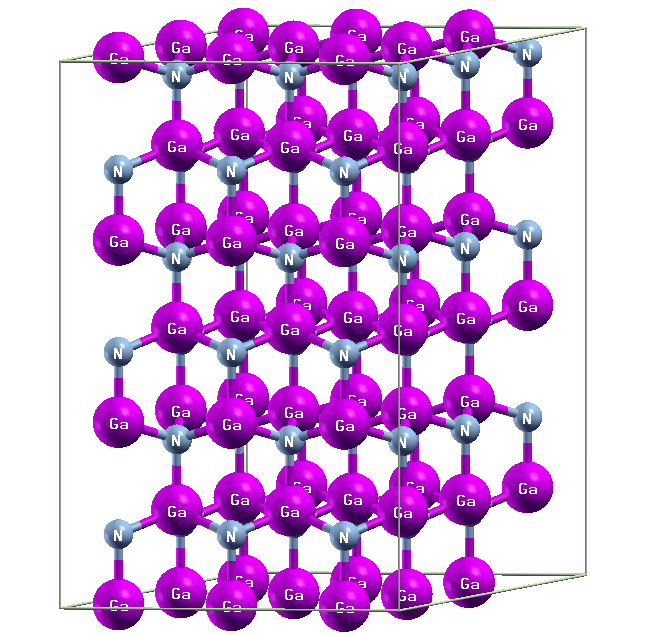
\includegraphics[scale=0.3]{images/GaN_3x3x3}
\par\end{centering}

\caption{GaN $3\times3\times3$ supercell}


\end{figure}


\texttt{cif2cell} has other options that you may want to explore.
You can find the help by issuing the following command

\begin{lstlisting}
cif2cell --help
\end{lstlisting}


\bibliographystyle{unsrt}
\bibliography{qe-tutor}

\end{document}
